\section{Aplicación Android} 
\subsection{Arquitectura Clean}
El escribir código de buena calidad puede resultar difícil por lo cual es necesario seguir ciertas reglas para lograr esto, es por eso que se utiliza la arquitectura Clean en android.

\begin{figure}[H]
        \centering
        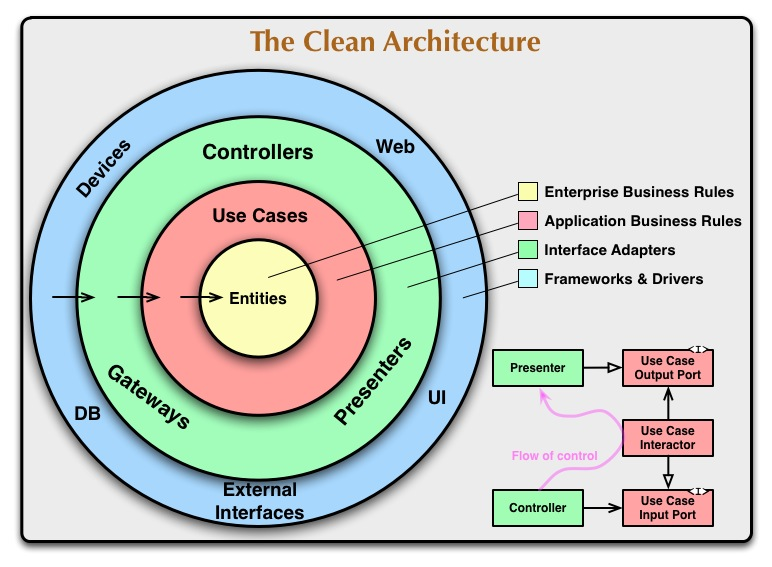
\includegraphics[width=0.7\textwidth]{capitulo2/android/img/cleanArquitectura.png}
        \caption{Arquitectura Clean \cite{cleanCodeBlog}} 
        \label{fig:cleanArquitectura}
\end{figure}

La arquitectura Clean como se muestra en la figura \ref{fig:cleanArquitectura} fue descrita por Robert C. Martin en 2012 y al utilizarla se puede llegar a tener las siguientes características en los sistemas \cite{cleanCodeBlog}:
\begin{itemize}
    \item Independientes de frameworks. El sistema no depende de las librerías o frameworks que se utilicen por lo que estas son fácilmente reemplazables.
    \item Que se puedan probar. Las reglas de negocio se pueden probar sin base de datos, interfaz de usuario, servidor web u otro elemento externo.
    \item Independientes de la interfaz de usuario. La interfaz de usuario puede cambiar fácilmente.
    \item Independientes de la base de datos. Las reglas de negocio no están ligadas a la fuente de datos por lo cual esta puede cambiar.
    \item Independencia de cualquier agente externo. Las reglas de negocio no dependen de otras capas, por lo cual se vuelve la parte más importante de la arquitectura.
\end{itemize}
%y todos sus componentes
    % UI fragments y actividades
    % MVVM
    % entidades
    % repository pattern
    % fuente de datos
\subsection{SOLID}
SOLID es un acrónimo que hace referencia a los cinco principios de la programación orientada a objetos, este acrónimo fue descrito por Robert C. Martin el seguir estos conceptos permite tener software que sea escalable y fácil de mantener, estos principios están ligados con la alta cohesión y bajo acoplamiento en el software. \cite{solidCode}
\paragraph{S-Responsabilidad simple} Cada clase debe de tener una sola responsabilidad. De no seguir esto puede generar el problema de que alguna clase tenga comportamiento que nada tiene que ver con ella debido a que dicho comportamiento no se aisló en otra clase diferente. \cite{solidEjemplos}
\paragraph{O-Abierto/Cerrado} Las clases, métodos y módulos deben de ser abiertos a la extensión pero cerrados en su modificación. Esto implica no reescribir código que ya se tiene si no crear nuevo código que haga uso de lo que ya se tiene desarrollado, una forma de hacer esto es hacer uso de la herencia o utilizar interfaces.\cite{solidEjemplos}
\paragraph{L-Sustitución Liskov} Las subclases nunca deben de romper la definición de la clase padre. Cuando se utiliza una clase y existen clases que heredan de dicha clase debe de ser posible el utilizar una de estas clases en lugar de la clase padre.\cite{solidEjemplos}
\paragraph{I-Segregación de la interfaz} Si algún método de una interfaz no es utilizado no se debe de obligar a tener que implementarlo. Eso indica que las interfaces deben de ser bastante especificas para no tener métodos innecesarios por lo cual es preferible tener muchas interfaces con pocos métodos a pocas interfaces con pocos métodos que no se utilicen.\cite{solidEjemplos}
\paragraph{D-Inversión de dependencias} Los módulos de alto nivel no deben de depender de los de bajo nivel. Ambos deben depender de abstracciones, a su vez, las abstracciones no dependen de los detalles sino al contrario. Con esto se logra que las clases no estén totalmente acopladas debido a que en caso contrario es difícil de mantener. \cite{solidEjemplos}
